\section{Linker}

\subsection{¿Qué es un linker?}
Un linker (enlazador) es una herramienta fundamental en el proceso de desarrollo de software. Actúa como un “ensamblador” de piezas de código y datos provenientes de diferentes fuentes para crear un único archivo de salida.

\subsection{¿Qué hace?}
Sus tareas principales son:

\begin{itemize}[noitemsep]
  \item \textbf{Combinación de secciones de código y datos:} Los archivos objeto (\texttt{.o}) generados por el ensamblador o el compilador contienen secciones como \texttt{.text} (código), \texttt{.data} (datos inicializados) y \texttt{.bss} (datos no inicializados). El linker toma todas las secciones homónimas de los distintos archivos y las une en una sola sección en el archivo de salida, siguiendo un script de linker (\texttt{link.ld}) o las reglas por defecto.
  
  \item \textbf{Resolución de símbolos:} Cuando el código referencia símbolos (por ejemplo, el nombre de una función como \texttt{\_start} o una etiqueta de datos como \texttt{msg}), el linker busca su definición entre todos los archivos objeto y bibliotecas de entrada. Luego sustituye cada uso simbólico por la dirección final donde ese símbolo ha sido colocado en el archivo de salida. Si falta una definición, se produce un error de “referencia no definida”; si hay definiciones duplicadas, un error de “definición múltiple”.

  \item \textbf{Relocalización:} Los archivos objeto contienen direcciones provisionales o relativas. El linker ajusta (o “parchea”) estas direcciones para que apunten a las ubicaciones finales en el ejecutable resultante, teniendo en cuenta la dirección base especificada en el script del linker (por ejemplo, \texttt{0x7C00} en un bootloader). Esto incluye tanto saltos internos como referencias a símbolos externos.

  \item \textbf{Generación del archivo de salida:} Finalmente, escribe el resultado combinado, resuelto y relocalizado en un archivo. El formato puede ser un ejecutable estándar del sistema operativo (ELF, PE) o, si se solicita explícitamente (con \texttt{--oformat binary}), una imagen binaria cruda sin cabeceras adicionales.
\end{itemize}

\section{¿Qué es la dirección 0x7C00 y por qué es necesaria?}

La dirección \texttt{0x7C00} es un estándar histórico en la arquitectura x86 que corresponde al punto de memoria física donde el BIOS carga el primer sector arrancable (MBR o VBR, 512 bytes) de un dispositivo seleccionado para el arranque. Su importancia y necesidad en el script del linker se sustenta en varios aspectos:

\begin{itemize}[noitemsep]
  \item \textbf{Convención del BIOS:} Cuando una PC compatible arranca en modo legado (BIOS o UEFI CSM), el firmware busca un dispositivo arrancable, lee su primer sector (512 bytes) y lo copia en la dirección física \texttt{0x7C00}. Inmediatamente después, establece los registros \texttt{CS:IP} a \texttt{0000:7C00} y salta a esa dirección para comenzar la ejecución.

  \item \textbf{Cálculo de direcciones finales:} El código ensamblado (\texttt{main.S}) incluye referencias a sus propias etiquetas (por ejemplo, la dirección de la cadena \texttt{msg} o el destino del salto \texttt{jmp print\_loop}). Para que esas referencias apunten a las ubicaciones correctas durante la ejecución (cuando el código resida en \texttt{0x7C00}), el linker *debe* conocer esta dirección base durante el proceso de enlace. Al indicar \texttt{. = 0x7C00} al principio de la sección \texttt{SECTIONS} en el script \texttt{link.ld}, le decimos al linker: “Considera que el inicio del código estará en \texttt{0x7C00} y calcula todas las direcciones relativas a esta base”.

  \item \textbf{Relocalización adecuada:} Gracias a esa directiva (\texttt{. = 0x7C00}), el linker puede calcular la dirección absoluta correcta para cada símbolo y referencia interna. Por ejemplo, si la etiqueta \texttt{msg} está a un desplazamiento de 26 bytes desde el inicio (\texttt{\_start}), el linker codificará su dirección como \texttt{0x7C00 + 26 = 0x7C1A} dentro de la instrucción \texttt{movw \$msg, \%si}.

  \item \textbf{Evitar desajustes catastróficos:} Si el linker no supiera la dirección de carga \texttt{0x7C00} (por ejemplo, si asumiera una base 0), calcularía todas las direcciones internas de forma incorrecta respecto al punto de carga real. Cuando el BIOS cargase el código en \texttt{0x7C00}, una instrucción como \texttt{movw \$msg, \%si} cargaría una dirección errónea (ej., 0x1A en lugar de 0x7C1A). El programa fallaría inmediatamente al intentar leer la cadena o realizar saltos, probablemente causando un cuelgue o reinicio.
\end{itemize}

\newpage % Inicia la sección práctica en una nueva página

\section{Demostración Práctica: Compilación, Enlace y Depuración}

Para ilustrar los conceptos anteriores, se realizó el proceso completo para crear, verificar y depurar un pequeño programa "Hello World" que funciona como un sector de arranque MBR en modo real de 16 bits.

\subsection{Compilación con el Ensamblador (as)}

El primer paso es convertir el código fuente en ensamblador (\texttt{main.S}, que contiene la directiva \texttt{.code16} para indicar que es código de 16 bits) en un archivo objeto (\texttt{main.o}).

\begin{lstlisting}[style=BashInputStyle, caption=Comando de ensamblaje inicial]
as -o main.o main.S
\end{lstlisting}

Sin embargo, al ejecutar esto en un sistema operativo host de 64 bits (como Ubuntu x86\_64), el ensamblador \texttt{as}, aunque genera las instrucciones correctas de 16 bits gracias a \texttt{.code16}, crea un archivo objeto ELF que internamente está marcado con la arquitectura \texttt{x86-64}. Esto causa conflictos posteriores con el linker cuando se intenta generar una salida \texttt{i386}.

Para mitigar esto, se puede intentar forzar a \texttt{as} a usar un formato más tradicional o directamente usar una Máquina Virtual Linux de 32 bits o un compilador cruzado (\textit{cross-compiler}) \texttt{i686-elf-as}. Una opción que a veces funciona es:
\begin{lstlisting}[style=BashInputStyle, caption=Intento de comando de ensamblaje (puede variar)]
as --traditional-format -o main.o main.S
\end{lstlisting}
(Nota: La solución más fiable para evitar estos problemas es usar una VM de 32 bits o un compilador cruzado.)

\subsection{Enlace con el Linker (ld)}

Una vez obtenido el archivo objeto \texttt{main.o}, se utiliza el linker \texttt{ld} junto con el script \texttt{link.ld} para generar la imagen binaria final \texttt{main.img}.

\begin{lstlisting}[style=BashInputStyle, caption=Comando de enlace]
ld -m elf_i386 -T link.ld -o main.img main.o
\end{lstlisting}

Explicación de las opciones:
\begin{itemize}[noitemsep]
    \item \texttt{-m elf\_i386}: Esencial para resolver conflictos de arquitectura. Indica a \texttt{ld} que procese la entrada y genere (internamente antes de convertir a binario) para la arquitectura \texttt{i386}. Asegura la compatibilidad con el objetivo y \texttt{OUTPUT\_ARCH(i386)} del script.
    \item \texttt{-T link.ld}: Especifica que se deben usar las reglas definidas en el archivo \texttt{link.ld}. Este script establece la dirección base en \texttt{0x7C00}, organiza las secciones \texttt{.text}, \texttt{.data}, etc., y asegura (mediante \texttt{.org}/\texttt{.word} en \texttt{main.S} o directivas del linker) que la imagen final tenga 512 bytes y la firma MBR \texttt{0xAA55} en los últimos dos bytes.
    \item \texttt{-o main.img}: Nombre del archivo de salida.
    \item \texttt{main.o}: Archivo objeto de entrada.
\end{itemize}
El resultado es el archivo \texttt{main.img}, una imagen binaria cruda de 512 bytes lista para ser arrancada.

\subsection{Verificación (objdump vs. hd)}

Para visualizar el trabajo de relocalización realizado por el linker, comparamos la salida del desensamblador sobre el archivo objeto con un volcado hexadecimal de la imagen binaria final.

\begin{lstlisting}[style=BashInputStyle, caption=Comandos de verificación]
objdump -d main.o
hd main.img 
# o hexdump -C main.img
\end{lstlisting}

Qué comparar:
\begin{itemize}[noitemsep]
    \item \textbf{Desensamblado (\texttt{objdump}):} Muestra las instrucciones máquina y sus direcciones relativas (usualmente desde 0) dentro del archivo objeto. Por ejemplo, para \texttt{movw \$msg, \%si}, muestra la instrucción y una dirección \textit{relativa} para \texttt{msg} (ej., \texttt{0x1a}). Los bytes hexadecimales codificarán esta dirección relativa (ej., \texttt{be 1a 00}).
    \item \textbf{Volcado Hexadecimal (\texttt{hd}):} Muestra los bytes crudos del archivo \texttt{main.img}. Al buscar la misma secuencia de bytes para \texttt{movw \$msg, \%si} (empezará con \texttt{be}), se observa que los bytes de la dirección \textit{han cambiado}. En lugar de \texttt{1a 00}, ahora se verá la dirección \textit{absoluta} calculada por el linker usando \texttt{0x7C00} como base (ej., \texttt{1a 7c}, correspondiente a \texttt{0x7C1A} en little-endian). Esta diferencia demuestra la relocalización.
    \item \textbf{Firma MBR:} En la salida de \texttt{hd}, se verifica que los dos últimos bytes del archivo (offsets \texttt{0x1fe} y \texttt{0x1ff}) son \texttt{55 aa}.
\end{itemize}

\subsection{Depuración con QEMU y GDB}

Finalmente, se depura la ejecución del MBR usando el emulador QEMU y el depurador GDB.

\subsubsection{Iniciar QEMU en modo depuración}

\begin{lstlisting}[style=BashInputStyle, caption=Lanzar QEMU esperando a GDB]
qemu-system-i386 -fda main.img -boot a -s -S
\end{lstlisting}
Explicación de las opciones:
\begin{itemize}[noitemsep]
    \item \texttt{-fda main.img}: Carga \texttt{main.img} como disquete A. (Ajustar ruta si es necesario).
    \item \texttt{-boot a}: Indica a QEMU arrancar desde el disquete A.
    \item \texttt{-s}: Inicia un servidor GDB en \texttt{localhost:1234}.
    \item \texttt{-S}: Congela la CPU al inicio, esperando que GDB se conecte y dé la orden de continuar.
\end{itemize}
QEMU se inicia pero queda pausado.

\subsubsection{Sesión de GDB}

Se abre otra terminal y se inicia GDB.

\begin{enumerate}[noitemsep]
    \item \textbf{Conectar a QEMU:}
        \begin{lstlisting}[style=GdbStyle]
(gdb) target remote localhost:1234 
        \end{lstlisting}
        Se establece la conexión. GDB muestra la dirección inicial (\texttt{0x0000fff0}) y una advertencia sobre la falta de un ejecutable especificado, lo cual es normal.
    
    \item \textbf{Cargar Símbolos (Opcional pero recomendado):} Para usar etiquetas del código fuente.
        \begin{lstlisting}[style=GdbStyle]
(gdb) file main.o
        \end{lstlisting}
        GDB podría mostrar una advertencia sobre incompatibilidad de arquitecturas entre el archivo \texttt{.o} (marcado como x86-64 por \texttt{as}) y el objetivo \texttt{i386} reportado por QEMU. Sin embargo, en la práctica, a menudo GDB logra cargar los símbolos de todas formas.


    \item \textbf{Establecer Arquitectura (¡CRUCIAL!):} Indicar a GDB que interprete el código como 16 bits.
        \begin{lstlisting}[style=GdbStyle]
(gdb) set architecture i8086
        \end{lstlisting}
        
    \item \textbf{Establecer Breakpoint Inicial:} Detener la ejecución al inicio de nuestro código MBR.
        \begin{lstlisting}[style=GdbStyle]
(gdb) b *0x7c00
        \end{lstlisting}
        
    \item \textbf{Iniciar Ejecución:} Decirle a GDB que deje correr a QEMU.
        \begin{lstlisting}[style=GdbStyle]
(gdb) c
Continuing.
        \end{lstlisting}
        QEMU simula el final del BIOS, carga \texttt{main.img} y salta a \texttt{0x7c00}, donde GDB detiene la ejecución debido al breakpoint.
        \begin{figure}[H]
            \centering
            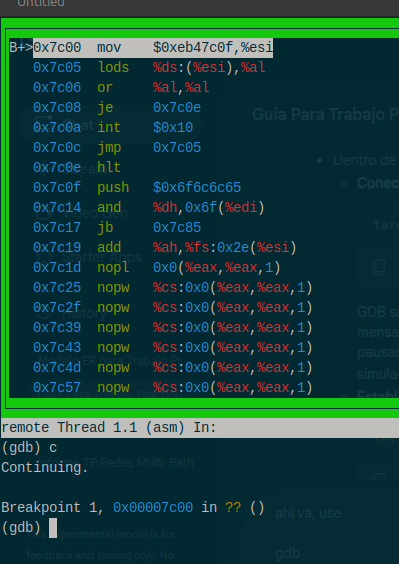
\includegraphics[width=0.8\textwidth]{images/break7C00.png}
            \caption{GDB detenido en el breakpoint en 0x7c00. Layout `asm` muestra el código.}
        \end{figure}

    \item \textbf{Ejecutar Paso a Paso y Observar:} Se utiliza \texttt{si} (Step Instruction) para avanzar instrucción por instrucción.
        \begin{itemize}
            \item Con \texttt{info registers} (o \texttt{layout regs}), se observa el cambio en los registros \texttt{ax}, \texttt{ds}, \texttt{es} (inicialización a 0) y \texttt{si} (carga de la dirección de \texttt{msg}).
              \begin{figure}[H]
                  \centering
                  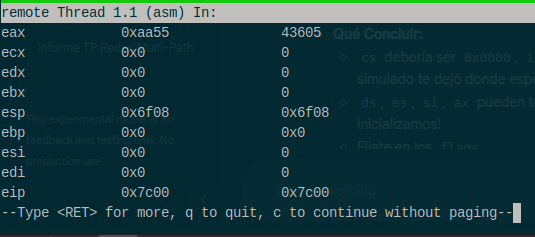
\includegraphics[width=0.8\textwidth]{images/registers7c00.png}
                  \caption{Salida parcial de `info registers` al inicio.}
              \end{figure}
            \item Se sigue el bucle \texttt{print\_loop}:
              \begin{figure}[H]
                  \centering
                  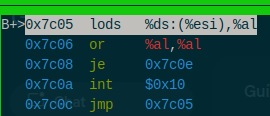
\includegraphics[width=0.6\textwidth]{images/bucle.png}
                  \caption{Instrucciones del bucle de impresión en GDB.}
              \end{figure}
              Se observa cómo \texttt{lods} carga un carácter en \texttt{al} e incrementa \texttt{si}. 
              Esa imagen representa el bucle donde se carga letra por letra el 'hello world'
        \end{itemize}

    \item \textbf{Correr hasta el Final:} Para ver el resultado completo:
        \begin{lstlisting}[style=GdbStyle]
(gdb) b halt # Poner breakpoint en la etiqueta halt
(gdb) c      # Continuar hasta halt
        \end{lstlisting}
        Se observa el mensaje completo en QEMU. GDB se detiene en la instrucción \texttt{cli} en \texttt{halt}.

    \item \textbf{Últimas Instrucciones:} Con \texttt{si}, se ejecuta \texttt{cli} (se verifica el flag \texttt{IF} desactivado con \texttt{info registers flags}) y luego \texttt{hlt}. Al ejecutar \texttt{hlt}, la CPU simulada se detiene. GDB ya no puede avanzar más. Se sale de GDB con \texttt{quit}.
    \begin{figure}[H]
        \centering
        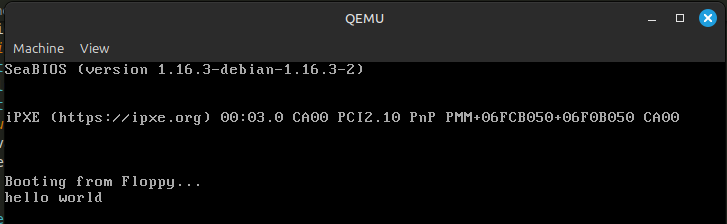
\includegraphics[width=0.8\textwidth]{images/resultado.png}
        \caption{Resultado final.}
    \end{figure}
\end{enumerate}
